\begin{frame}{Les prépositions \gloss{Prepositions}}
  \begin{columns}
    \column{0.5\textwidth}
      Je vais... (à)
      \begin{enumerate}
        \item \underline{\uncover<2->{à la}} gare.
        \item \underline{\uncover<4->{au}} gymnase.
        \item \underline{\uncover<6->{aux}} théâtres.
      \end{enumerate}
      J'arrive... (de)
      \begin{enumerate}
        \setcounter{enumi}{3}
        \item \underline{\uncover<8->{des}} piscines.
        \item \underline{\uncover<10->{de la}} librairie.
        \item \underline{\uncover<12->{du}} musée.
      \end{enumerate}
    \column{0.5\textwidth}
      \begin{minipage}[c][0.6\textheight]{\linewidth}
        \begin{center}
          \only<-2>{
            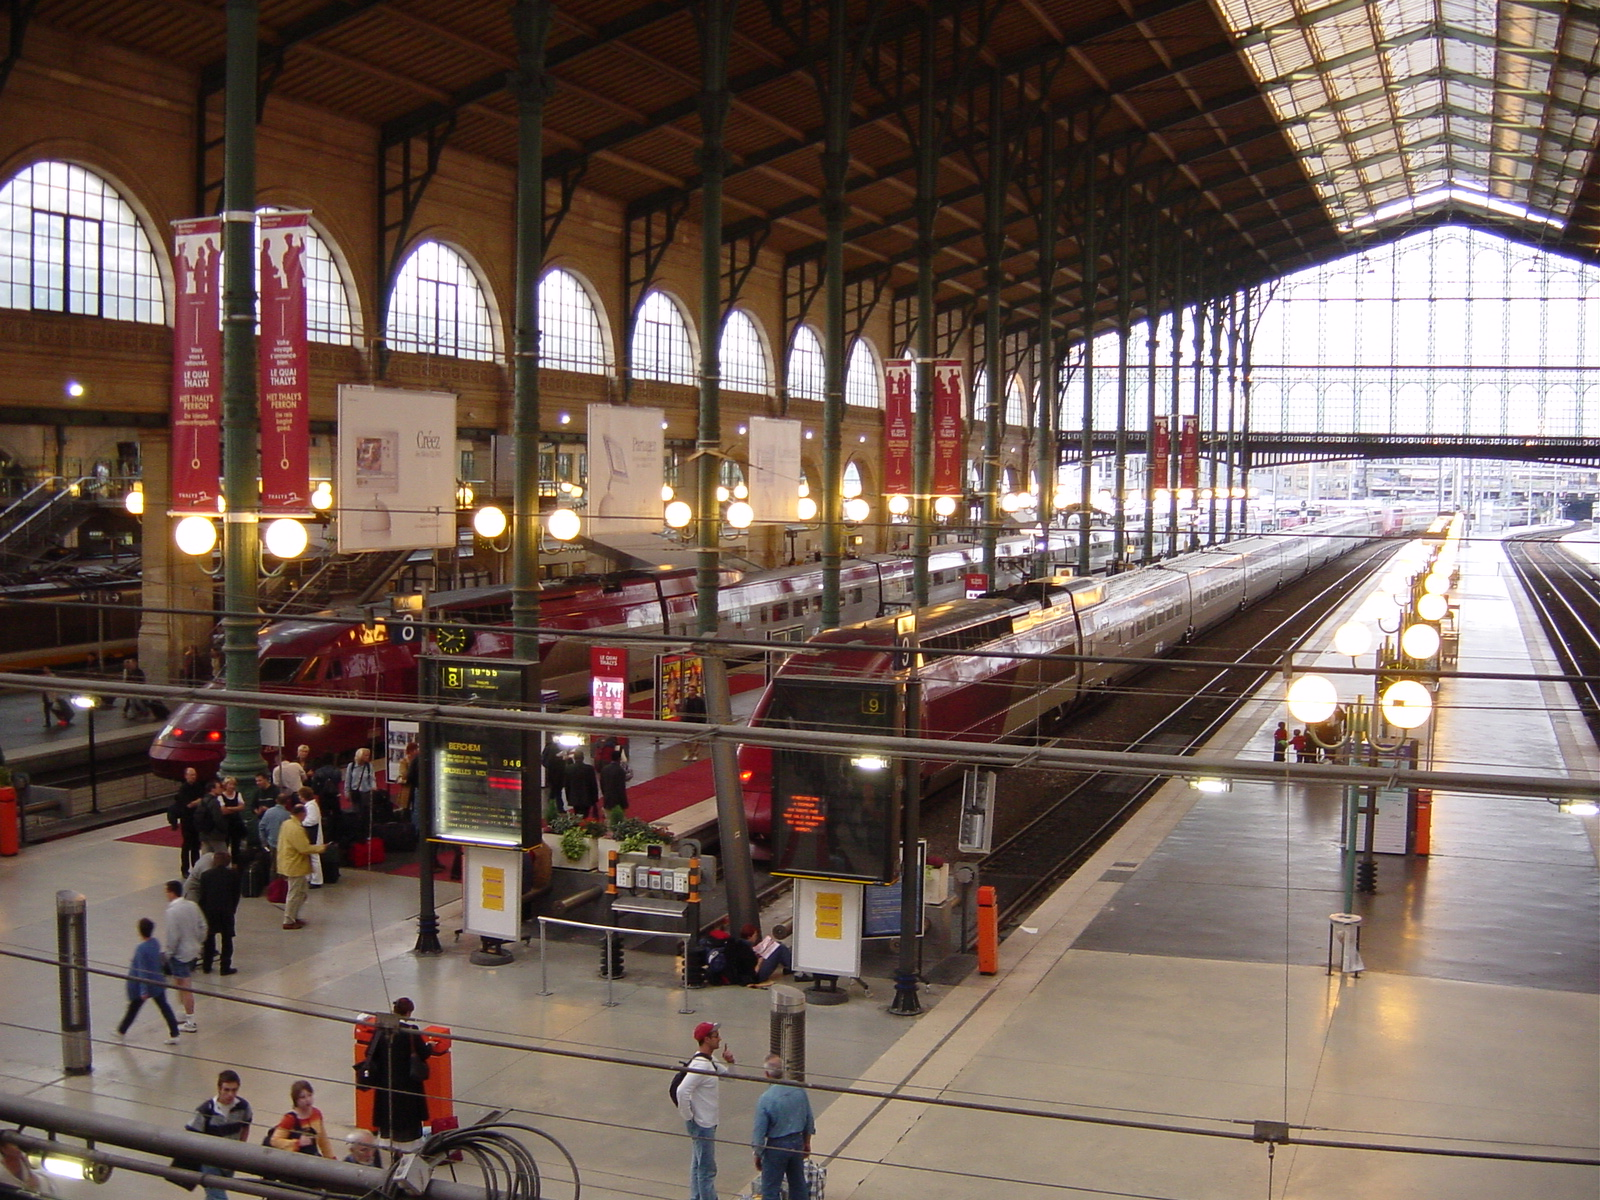
\includegraphics[scale=0.1]{gare_du_nord.jpg}
          }
          \only<3-4>{
            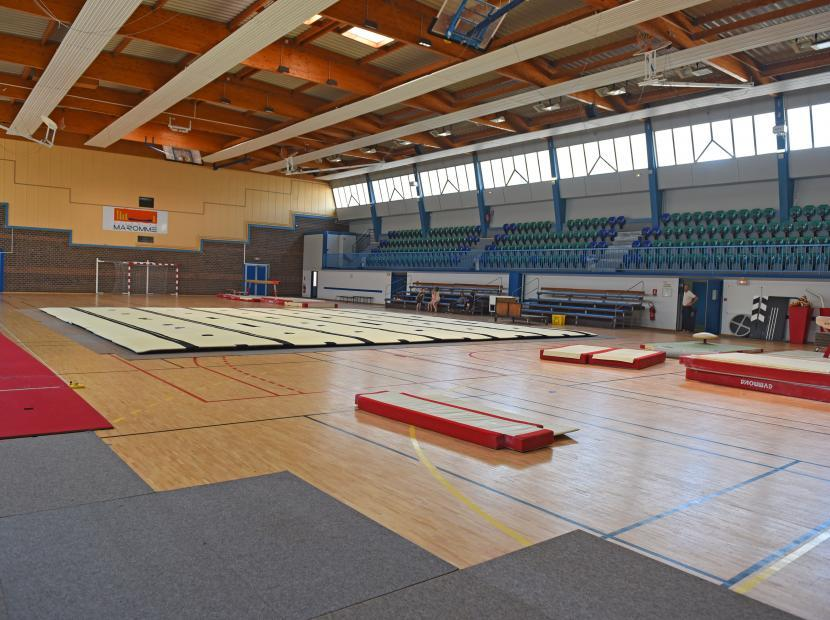
\includegraphics[scale=0.16]{gymnase.jpg}
          }
          \only<5-6>{
            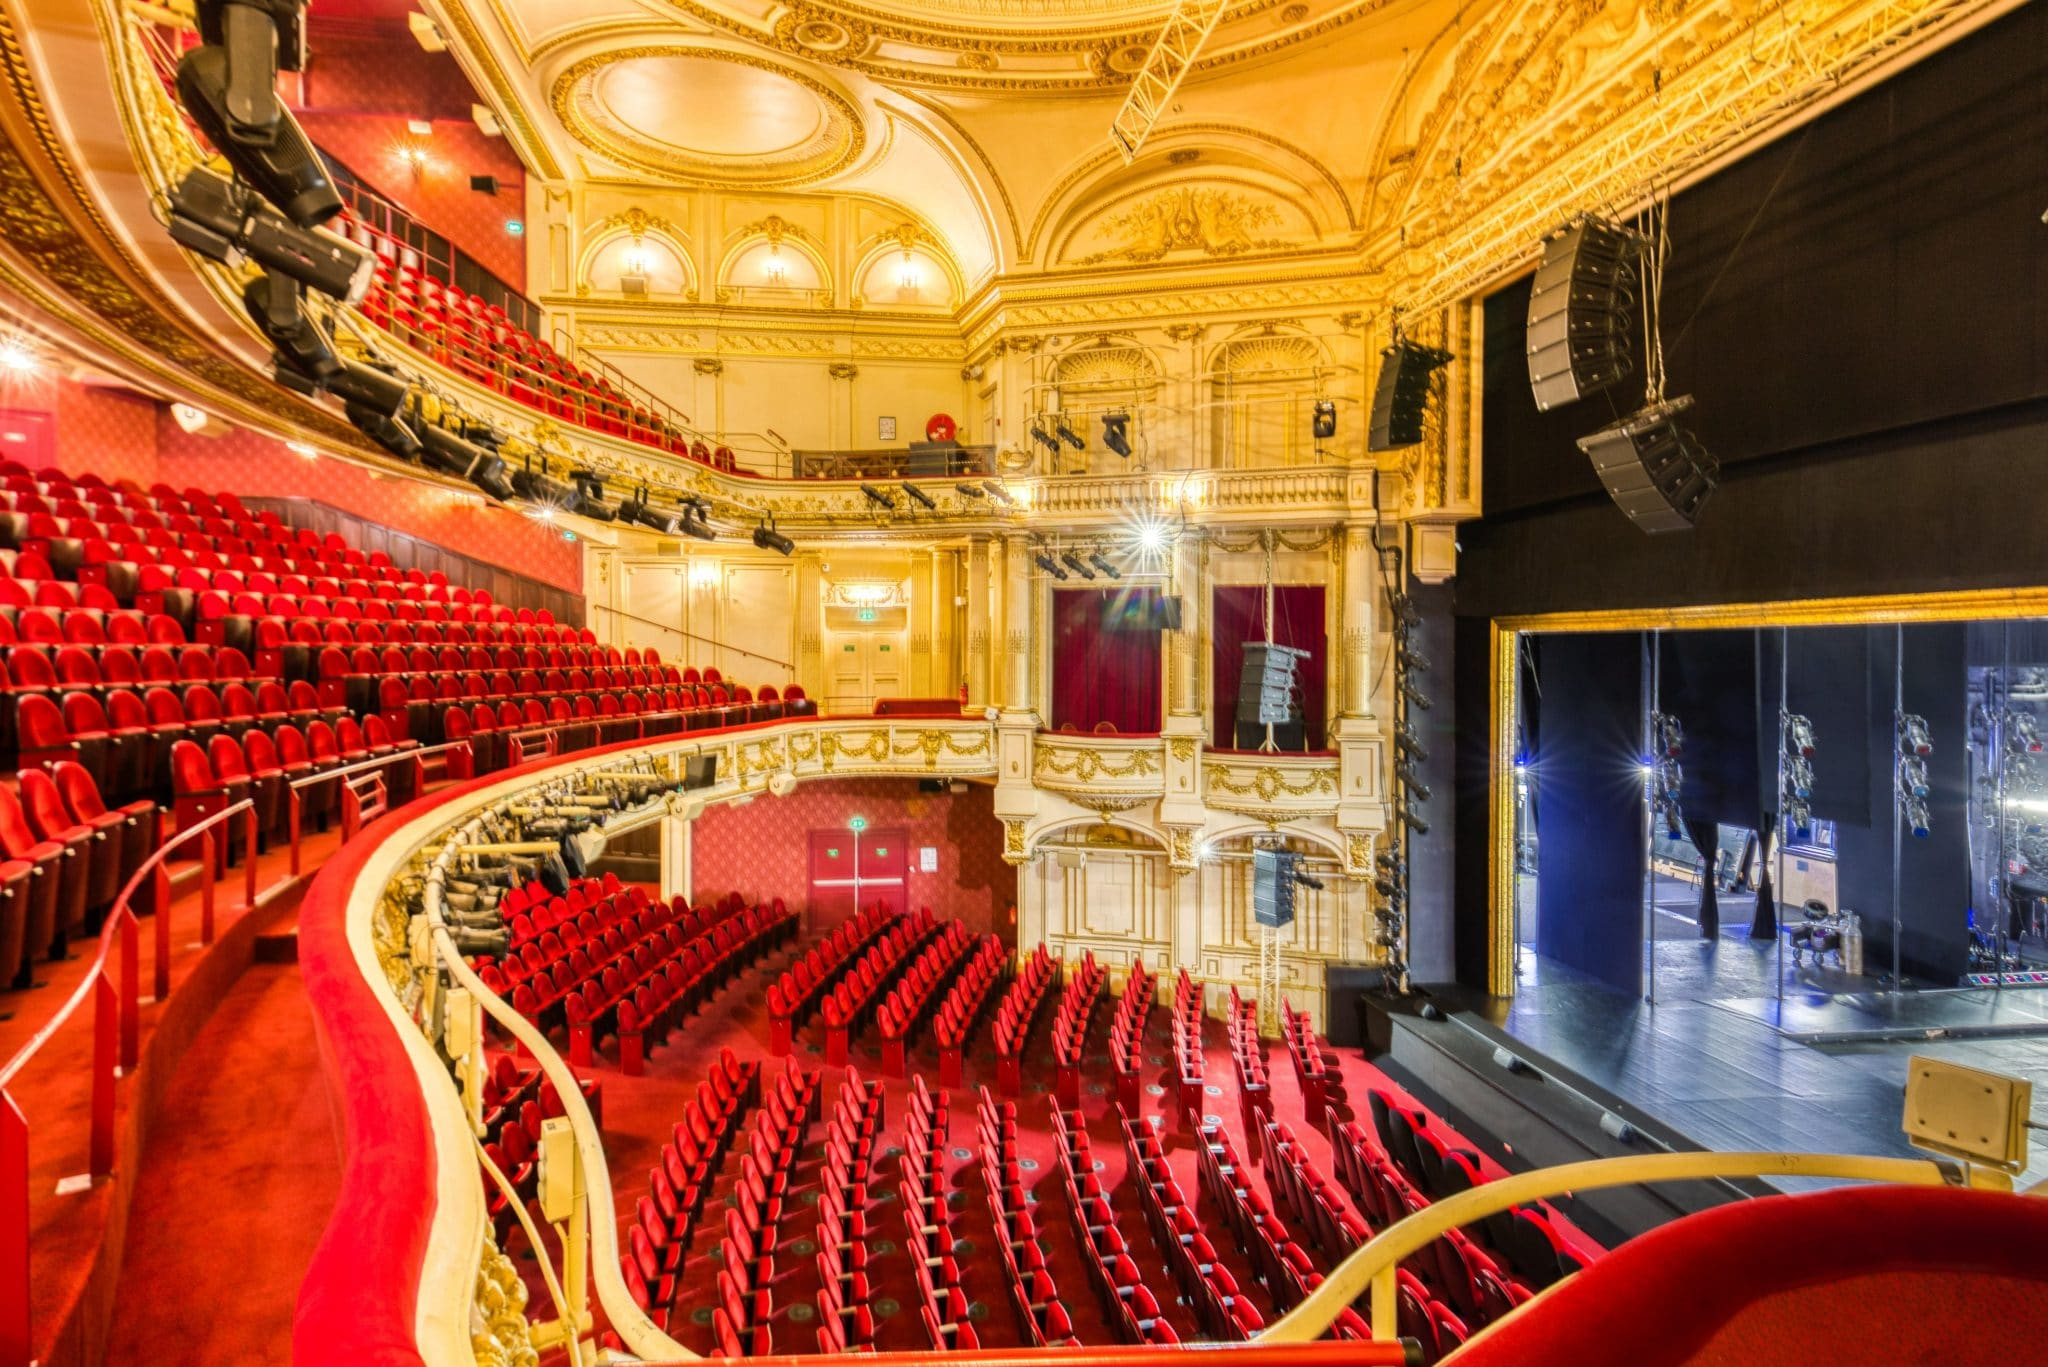
\includegraphics[scale=0.08]{theatre.jpg}
          }
          \only<7-8>{
            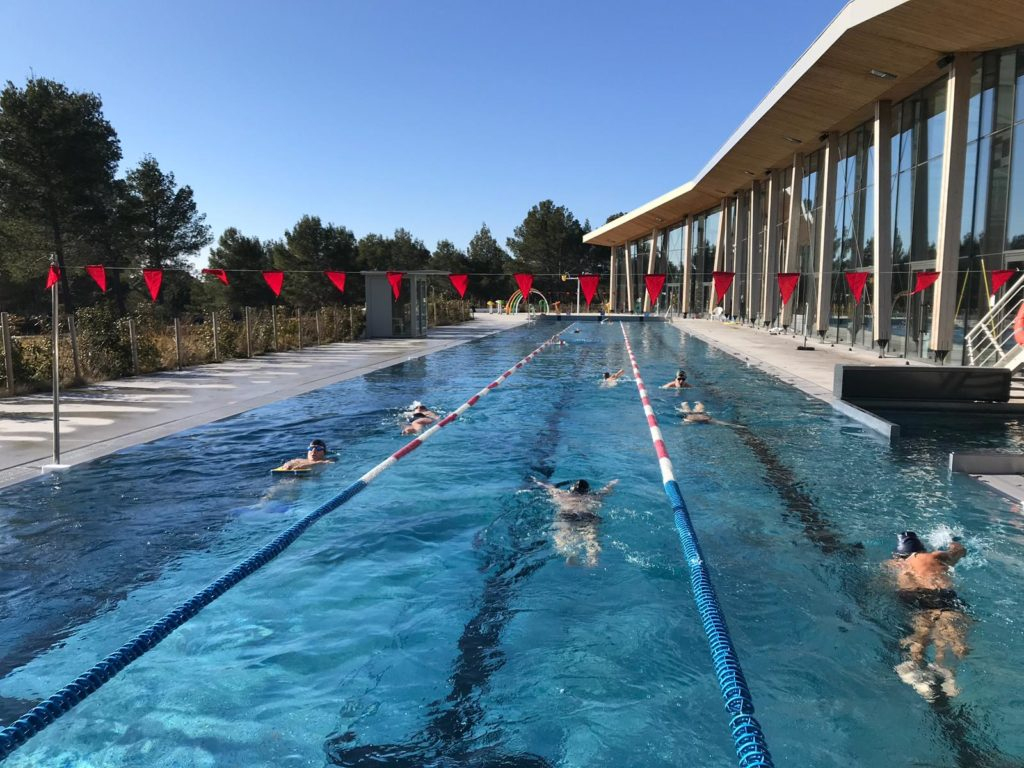
\includegraphics[scale=0.22]{piscine.jpeg}
          }
          \only<9-10>{
            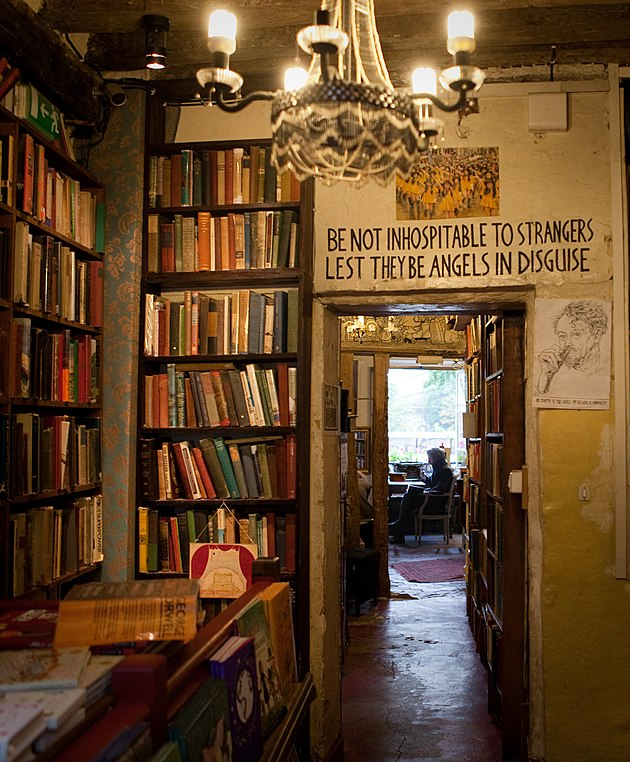
\includegraphics[scale=0.23]{librairie.jpg}
          }
          \only<11-12>{
            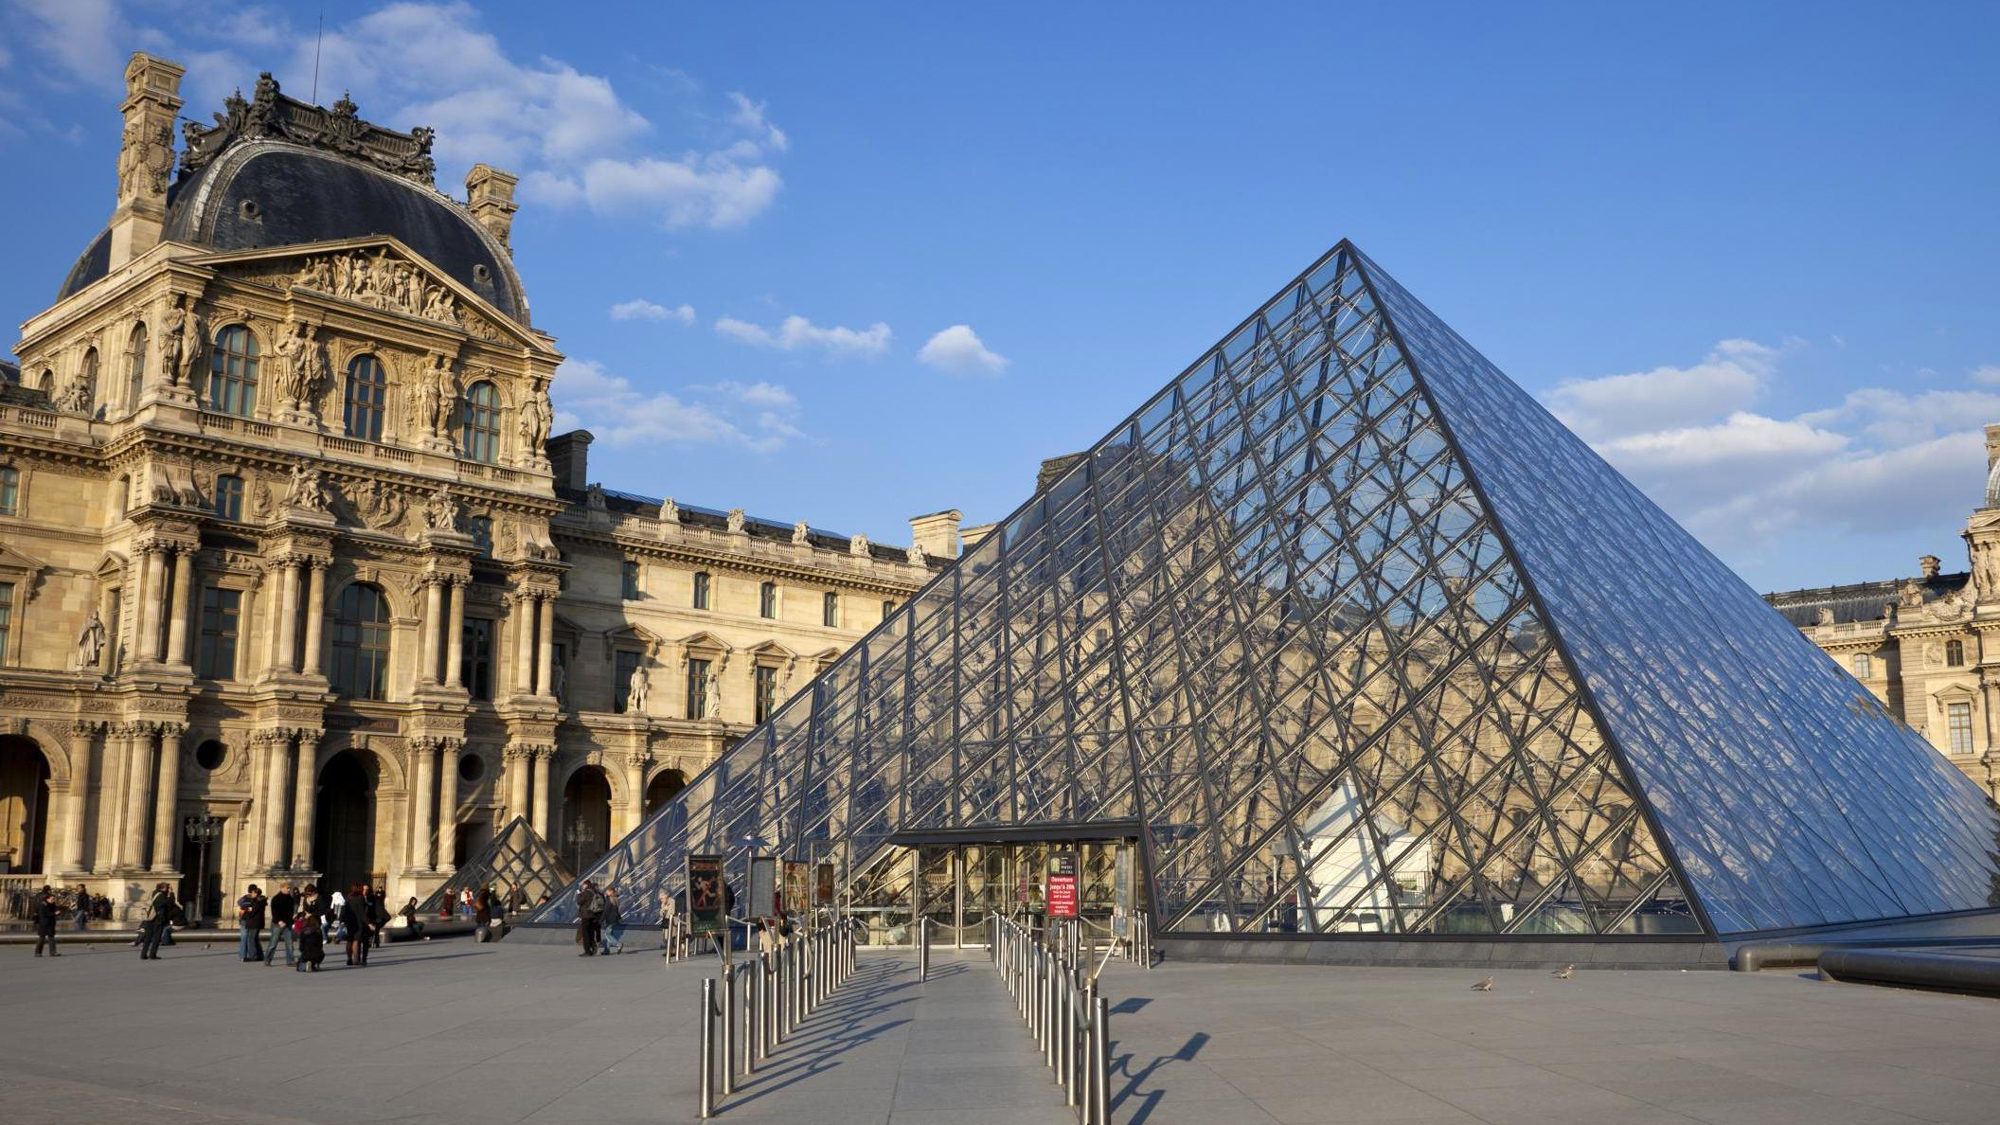
\includegraphics[scale=0.08]{louvre.jpg} \\
            Le Louvre à Paris
          }
        \end{center}
      \end{minipage}
  \end{columns}
\end{frame}